\chapter[Algoritmo proposto]{Algoritmo proposto}
\label{chapter_macod}

O algoritmo proposto neste trabalho é baseado em colônia de formigas (ACO) e foi chamado de \textit{Many-objective Ant Colony Optimization based on Non-Dominated Sets} (MACO/NDS), em português, otimização em colônia de formigas para muitos objetivos baseada em decomposição de feromônios \cite{Franca2018}. A proposição envolve os seguintes módulos:

\begin{itemize}
	\item Modelo PMM: construção da solução para o problema da mochila multiobjetivo, apresentado na seção \ref{section_algoritmo_pmm}.
	\item Modelo PRM: construção da solução para o problema do roteamento multicast, apresentado na seção \ref{section_algoritmo_prm}.
	\item \textit{Framework} ACO: algoritmo geral voltado à manipulação de problemas \textit{many-objective} desenvolvido para se trabalhar com qualquer problema discreto, apresentado na seção \ref{section_algoritmo_framework}.
\end{itemize}

Este capítulo apresenta a construção da solução no ACO para ambos os problemas (PMM e PRM). Os modelos de construção, apesar de terem sido propostos para o MACO/NDS, podem ser utilizados em qualquer algoritmo ACO. O \textit{framework} MACO/NDS, componente principal do algoritmo, é descrito em seguida na seção \ref{section_algoritmo_framework}. Nela são discutidos alguns conceitos gerais sobre a implementação multiobjetivo do ACO, bem como uma descrição mais detalhada das etapas de construção das soluções e atualização dos feromônios.

\section{Construção da solução para o PMM}
\label{section_algoritmo_pmm}

Como mostrado na seção \ref{section_representacao_pmm}, os AGs utilizam vetores binários para representar as soluções do PMM. Nos ACOs, é possível utilizar a mesma representação, entretanto, deve-se desenvolver um algoritmo que constrói a solução a partir de uma estrutura de feromônios e uma heurística. O processo de gerar as soluções é mais simples nos AGs, pois basta efetuar as operações de \textit{crossover} e mutação sobre os vetores binários. No entanto, a implementação de um ACO para o PMM pode ser desafiadora, já que as colônias de formigas foram inicialmente propostas para lidar com grafos e não vetores de bits. Diversos trabalhos que adotam ACOs para a resolução do problema da mochila são encontrados na literatura \cite{Ke2010,kong2008,changdar2013,Alaya2004,Alaya2007}.

As colônias de formigas foram propostas inicialmente para problemas em grafos, e, portanto, não é intuitivo sua adaptação para outros tipos de problemas, como o problema do mochila. Entretanto, como mostrado em \cite{Ke2010}, não é necessário ter um grafo para se utilizar a técnica, sendo possível manipular os feromônios de diversas outras formas. Foram encontradas na literatura três diferentes formas de lidar com os feromônios para o problema da mochila multiobjetivo (PMM). A primeira abordagem consiste em depositar feromônios em cada um dos itens \cite{Leguizamon1999}. Sempre que um item é escolhido para compor a solução, incrementa-se a quantidade de feromônios presente no item. Dessa forma, a quantidade de feromônio em cada item representa sua preferência em relação aos demais. A segunda abordagem propõe a criação de um grafo direcionado que representa a preferência em incluir um item $b$ após a inclusão do item $a$ \cite{Fidanova2003}. Dessa forma, sempre que se escolher um item $a$ e posteriormente um $b$, deposita-se feromônio na aresta $(a,b)$ do grafo. Ao construir uma solução, analisa-se o último item selecionado e todas as arestas no grafo que partem dele. O destino com a maior quantidade de feromônios representa o item preferível. A terceira estratégia foi proposta por \cite{Alaya2004} e utiliza um conceito de aresta semelhante à abordagem anterior. Entretanto, ao invés de depositar feromônios apenas em pares consecutivos, eles são depositados para todos os pares de objetos existentes na solução. Por exemplo, se na solução os itens $a$, $d$ e $f$ estão na mochila e no passo atual adiciona-se o item $c$, o depósito de feromônios é feito nas arestas $(a,c)$, $(d,c)$ e $(f,c)$, de forma que o grafo represente a preferência de se escolher um item dado que algum outro item já tenha sido selecionado. Assim, ao construir a solução, deve-se analisar todas as arestas com origem em algum item já presente na solução, o destino da aresta com maior quantidade de feromônios representa o item mais desejável. Neste trabalho utilizou-se a primeira estratégia que deposita os feromônios diretamente nos itens.

Além dos feromônios, outra importante fonte de informação para se construir uma solução no ACO é a heurística. Ela é responsável por estimar o quão vantajoso é escolher um item em relação a outro. Tomando como inspiração o estudo de \cite{Ke2010}, a implementação do ACO para o PMM utiliza como heurística o seguinte modelo de funções:

\begin{itemize}
	\item Para cada objetivo $k$ (lucro do item), cria-se uma função de heurística $h_k$ que recebe dois parâmetros, a capacidade restante ($cr$) e o item que se deseja incluir. A capacidade restante é a diferença entre a capacidade da mochila e a soma dos pesos dos itens que já foram incluídos. A heurística é então dada por: \begin{equation}h_k(item, cr) = lucro_k(item) \times (1 - \frac{peso(item)}{cr})\end{equation}
	\item Uma heurística extra é usada exclusivamente para se referir ao peso do item, a qual é dada por: \begin{equation}h_{peso}(item) = 1 - \frac{peso(item)}{peso\_maximo}\end{equation}
\end{itemize}

Logo, o número de heurísticas no PMM, por item, é sempre o número de objetivos + 1. Tendo definido a estrutura de feromônios e as heurísticas, para construir uma solução, o algoritmo recebe a função heurística ($h$) e um vetor de feromônios ($\tau$). A heurística $h$ é normalmente uma combinação de todas as heurísticas. No caso do MACO/NDS, $h$ é uma média ponderada das heurísticas $h_1, h_2, .., h_k$ e $h_{peso}$, esse processo é detalhado na Seção \ref{section_macod_solutions}.

Para escolher o próximo item da solução, uma formiga analisa todas as possibilidades e então toma uma decisão com base nas probabilidades indicadas pelos feromônios e pelas heurísticas. Para avaliar as possibilidades, utiliza-se uma lista de exploração $Exp$. A lista de exploração $Exp$ contém todos os itens possíveis, a probabilidade $p$ de cada item $exp_i \in Exp$ é calculada de acordo com a heurística de $exp_i$ ($h(exp_i)$) e a quantidade de feromônios no item $\tau_i$, como mostrado na fórmula a seguir:

\begin{equation}p(exp_i) = \frac{\tau_i^\alpha + h(exp_i)^\beta}{\sum_{j \gets 0}^{tamanho(Exp)} \tau_j^\alpha + h(exp_j)^\beta}\end{equation}

O próximo item na solução é escolhido de acordo com as probabilidades calculadas em uma espécie de roleta, onde, quanto maior o valor de probabilidade ($p(exp_i)$), maior a chance do item ser escolhido. Após ter selecionado um item, recalcula-se a lista $Exp$ para que contenha apenas itens válidos para a solução, isto é, remove-se qualquer elemento de $Exp$ que, se incluído na solução, excede a capacidade da mochila. O processo é repetido até que $Exp$ seja uma lista vazia.

A fim de reduzir a complexidade do algoritmo de construção da solução para o PMM, ao invés de se utilizar a lista completa de itens possíveis ($Exp$), utiliza-se uma amostra desse conjunto ($Exp'$). $Exp$ é calculado normalmente, mas ao submeter-se o conjunto para o cálculo de probabilidades e roleta, no lugar de $Exp$, é utilizado $Exp'$, uma amostra aleatória de tamanho fixo $Exp'_{size}$ (parâmetro do algoritmo) da lista completa $Exp$.

\section{Construção da solução para o PRM}
\label{section_algoritmo_prm}

A modelagem de um algoritmo genético para o problema do roteamento multicast não é trivial, pois deve-se representar os caminhos entre o servidor e os múltiplos destinos em uma rede de computadores, ou seja, uma árvore. Em contrapartida, o PRM se aproxima da definição original do ACO, pois trabalha com grafos. Dessa forma, a modelagem para o ACO do PRM é mais natural que a modelagem para o AG.

O processo de construção da solução para um ACO do PRM deve gerar a árvore \textit{multicast} com base no grafo da rede, da estrutura de feromônios e da heurística. Existem diversas maneiras de se criar tal árvore. A fim de estudar o comportamento das diferentes estratégias possíveis, aprimorá-las e determinar o melhor modelo para se utilizar no PRM, analisou-se o comportamento de cada ideia no caso mais básico possível: o PRM mono-objetivo. As ideias consideradas neste trabalho são listadas a seguir:

\begin{enumerate}
	\item A primeira estratégia, apresentada em \cite{Pinto2005}, pode ser vista como uma formiga que caminha pelo grafo até encontrar todos os destinos. A análise é feita passo a passo, considerando apenas a vizinhança do vértice corrente como possibilidades para compor a solução. O processo inicia com uma lista de exploração de vértices ($Exp_v$) que contém um único elemento: a raiz. Sorteia-se um vértice $i \in Exp_v$ e atribui-se probabilidades a todas as arestas $(i, j)$, onde $j$ é qualquer vértice não-visitado na adjacência de $i$, sendo que $i$ é removido de $Exp_v$ caso não possua vizinhos factíveis. Um vértice $v$ é escolhido de acordo com as probabilidades calculadas (conforme à seção \ref{section_otimizacao_aco_construcao}), a aresta $(i, v)$ é adicionada à solução e $v$ é inserido na lista de exploração $Exp_v$. O processo é repetido até que todos os destinos tenham sido alcançados. Como etapa final, poda-se a árvore, eliminando as folhas que não representam destinos.
	\item A segunda estratégia, até onde se sabe, proposta neste trabalho, manipula de forma independente os caminhos entre a raiz e cada um dos destinos. Portanto, nessa estratégia, $|D|$ formigas partem da raiz e, com base nas heurísticas e feromônios, encontram, cada uma, um vértice $d \in D$ diferente, sendo $D$ o conjunto de nós destinos. Com os caminhos para todos os nós destinos definidos, monta-se a árvore evitando a ocorrência de ciclos. Por fim, realiza-se a poda da árvore para excluir qualquer vértice folha que não seja um destino. %mants
	\item Uma terceira estratégia é proposta neste trabalho. Ela adota uma representação de formiga fictícia que pode estar em vários locais do grafo ao mesmo tempo (formiga com sobreposição quântica). Dessa forma, é possível analisar as probabilidades de todas as arestas factíveis ao mesmo tempo, ao invés de sempre escolher a composição da solução de acordo com uma vizinhança local. Ao considerar todas as possibilidades ao mesmo tempo, obtém-se um processo melhor de decisão que não apresenta qualquer tendência (viés) para algum dos ramos da árvore, já que, a todo momento, qualquer vértice factível pode ser incluído no resultado. O processo é iniciado a partir de uma lista de exploração de arestas ($Exp_a$) que contém todas as arestas conectadas ao nó raiz. A cada passo, calcula-se as probabilidades para toda aresta de $Exp_a$ e, de acordo com os valores obtidos, escolhe-se $exp_i \in Exp_a$ para compor a solução. $exp_i$ é então removida de $Exp_a$, adicionada à solução e tem todas suas arestas adicionadas à lista de exploração, desde que ainda não tenham sido incluídas. O processo é repetido até que todos os destinos sejam atingidos. Uma poda é realizada ao final do processo. Uma outra analogia para esse processo seria imaginar que a formiga é clonada sempre que visita um vértice. Dessa forma, haverá uma formiga em cada vértice já visitado e então a vizinhança de todos eles será considerada ao mesmo tempo.
	\item A última estratégia, também proposta e avaliada neste trabalho, consiste em construir a solução de forma inversa. Ao invés de partir da raiz e chegar aos destinos, este modelo propõe que se utilizem $|D|$ formigas, onde cada uma tem como posição inicial um nó destino $d \in D$ diferente. A ideia é que as formigas escolham seus caminhos localmente com base nas probabilidades das arestas em suas vizinhanças. Sempre que uma formiga encontrar o caminho que já foi explorado por outra formiga, ela para de explorar e segue os mesmos passos realizados pelo outro agente. O processo termina quando o nó raiz foi encontrado por alguma formiga e todas as formigas tiverem se encontrado em algum vértice. Em outras palavras, o processo inicia com uma componente conexa para cada $d \in D$. Em todo passo do algoritmo, cada componente conexa é explorada a partir do último nó adicionado. Nesse processo, calculam-se as probabilidades das arestas na vizinhança do nó explorado e escolhe-se, de acordo com os valores obtidos, um novo vértice $v$ para ser adicionado à componente. Se não há arestas factíveis na vizinhança, deve-se retroceder para um vértice anterior. Caso o nó incluído $v$ pertença a uma outra componente conexa, elas se unem. O processo termina quando existe apenas uma componente conexa e o vértice raiz foi encontrado. Por fim, uma poda é realizada como pós-processamento da árvore. 
\end{enumerate}

Cada uma das estratégias mencionadas foi implementada e avaliada a fim de determinar aquela que produz as soluções de melhor qualidade para o PRM. Para obter um valor como referência de qualidade, também foi implementada uma versão modificada do algoritmo de Prim \cite{Prim1957} que aproxima a árvore \textit{multicast} de menor custo. Como esperado, o algoritmo de Prim modificado, apesar de nem sempre conseguir os melhores resultados, é a opção mais rápida. Entretanto, a intenção deste estudo não é produzir um algoritmo melhor para o problema mono-objetivo, mas avaliar as estratégias de construção de solução com o objetivo de escolher aquela que será empregada em versões mais complexas (multiobjetivo) do PRM.

Os resultados dos experimentos, que podem ser encontrados na seção \ref{section_experimentos_etapa2}, mostram que nossa estratégia (formiga com sobreposição quântica) representa a melhor relação entre qualidade do resultado e tempo de execução. Portanto, para todos os demais experimentos no PRM, foi o método de construção da solução utilizado.

Durante a implementação da estratégia, foram adotadas algumas técnicas de amostragem a fim de agilizar o algoritmo, sem afetar significativamente a qualidade das soluções. O fluxograma apresentado na \autoref{fig_fuxo_construcao_solucao} mostra, de maneira geral, o funcionamento do algoritmo. A descrição detalhada dessa implementação é apresentada no Algoritmo \ref{alg_aco_prm_construir_solucao}, que recebe como parâmetros de entrada:

\begin{itemize}
	\item $G$: o grafo que representa a rede;
	\item $r$: o nó raiz, servidor de onde parte a mensagem;
	\item $D$: conjunto de nós destinos;
	\item $\tau$: estrutura de feromônios;
	\item $h$: função heurística;
	\item $Exp'_{size}$: tamanho da amostra.
\end{itemize}

\begin{figure*}[!htbp]	
	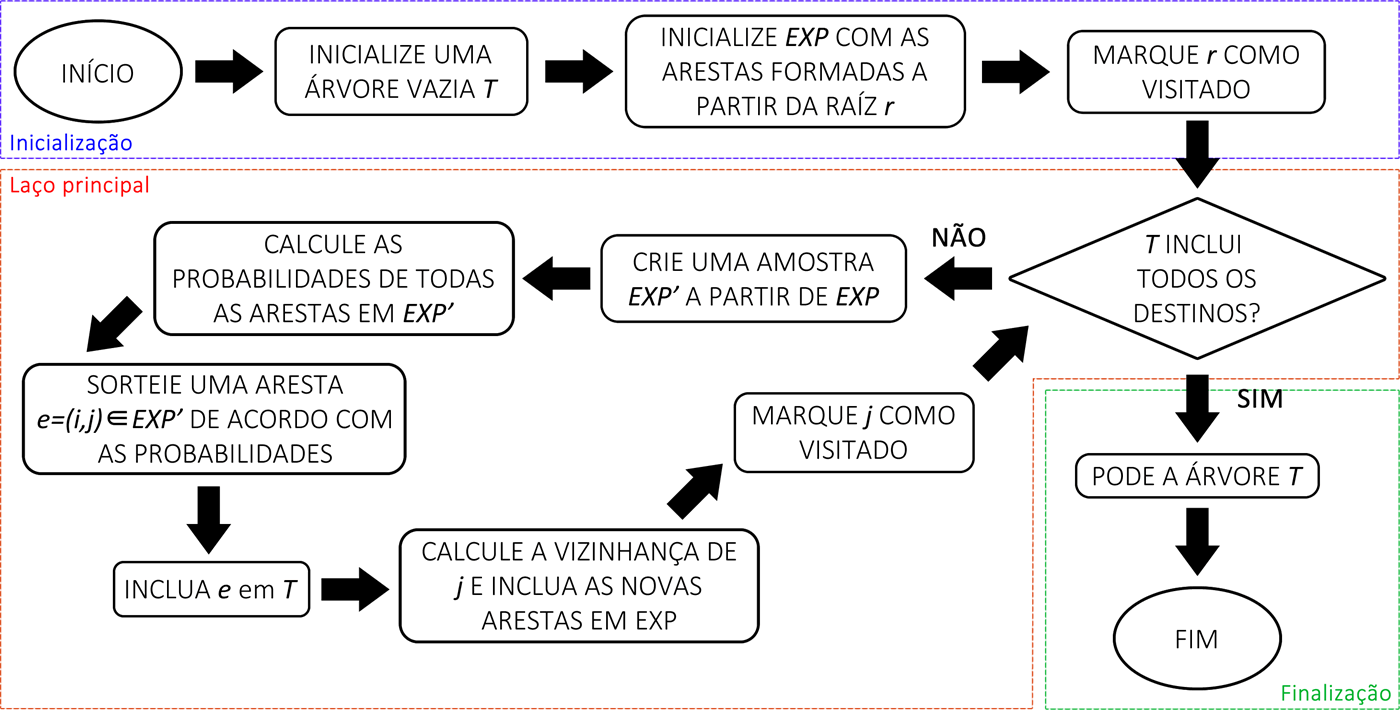
\includegraphics[width=1\textwidth]{cap_algoritmo-proposto/figs/fluxo-construcao-solucao}
	\caption{\label{fig_fuxo_construcao_solucao}Método de construção de soluções do ACO para o PRM}
\end{figure*}

\begin{algorithm}
	\caption{Geração de solução no ACO $(G, r, D, \tau, h, Exp'_{size})$}
	\label{alg_aco_prm_construir_solucao}
	\begin{algorithmic}[1]
		\State Inicie uma árvore vazia $T$
		\State Inicie $Exp_a$ com todas as arestas que possuem alguma extremidade em $r$
		\State Marque $r$ como visitado
		\While{$T$ não incluir todos os vértices em $D$}
		\State Crie uma amostra aleatória $Exp'$ a partir da lista $Exp_a$ com $Exp'_{size}$ elementos
		\State Calcule as probabilidades de todas as arestas em $Exp'$ de acordo com $\tau$ e $h$
		\State Escolha uma aresta $e=(i,j) \in Exp'$ de acordo com as probabilidades
		\State Inclua $e$ em $T$
		\State Marque $j$ como visitado
		\State Calcule a vizinhança $V$ do vértice $j$
		\For{$v \in V$}
		\If{já existe aresta $a$ em $Exp_a$ que leva a $v$}
		\State Remova $a$ de $Exp_a$
		\State Calcule as probabilidades de $a$ e de $(j, v)$ de acordo com $\tau$ e $h$
		\State Sorteie uma das duas arestas de acordo com as probabilidades e adicione a vencedora em $Exp_a$
		\ElsIf{$v$ não tiver sido visitado}
		\State Inclua $(j, v)$ em $Exp_a$
		\EndIf
		\EndFor
		\EndWhile
		\State Pode a árvore $T$
		\State \Return $T$
	\end{algorithmic}
\end{algorithm}

Um exemplo gráfico considerando um PRM simples é mostrado na \autoref{fig_exemplo_solucao}. No grafo apresentado na figura, $A$ é o vértice raiz, enquanto $\{B, D, F, G\}$ são os destinos. No passo 1, a formiga é colocada na raiz ($A$) e os vértices na vizinhança de $A$ se tornam candidatos a fazerem parte da árvore. Em cada passo a formiga escolhe o caminho a perseguir de acordo com os feromônios, a heurística e uma função de probabilidade. Em nosso exemplo, esse processo não é ilustrado, sendo apresentado apenas o caminho escolhido. No passo 2, a formiga escolhe o vértice $B$ e passa a enxergar a vizinhança de $B$ como candidata, mas diferentemente de métodos tradicionais, não deixa de considerar os vértices descobertos em $A$. Ainda no passo 2, verifica-se que o vértice $C$ pode ser atingido tanto por $A$ quanto por $B$. Este algoritmo não mantém duas arestas que levam ao mesmo destino, portanto uma delas deve ser retirada da lista de candidatos. Tal escolha é feita de acordo com o cálculo de probabilidade. Por exemplo, considerando que a aresta $(A, C)$ tem uma probabilidade menor que a aresta $(B, C)$, ela é  removida. No passo 3, a formiga escolhe ir para $C$ e agora enxerga toda a vizinhança de $A$, de $B$ e de $C$. No passo 4, dentre os vértices $\{D, E, F, G\}$ a formiga escolhe partir para $D$. No passo 5, a formiga adiciona a aresta $(A, G)$ à solução e, como no passo 2, a aresta $(G, F)$ é escolhida em detrimento da $(C, F)$, que é removida da exploração. No último passo, a formiga, que neste momento enxerga os vértices $\{E, F\}$ escolhe ir para $F$. Como todos os destinos foram adicionados à árvore, o processo termina. Em problemas mais complexos, pode ser necessário realizar uma poda, mas neste caso, a solução está completa.

\begin{figure*}[!htbp]	
	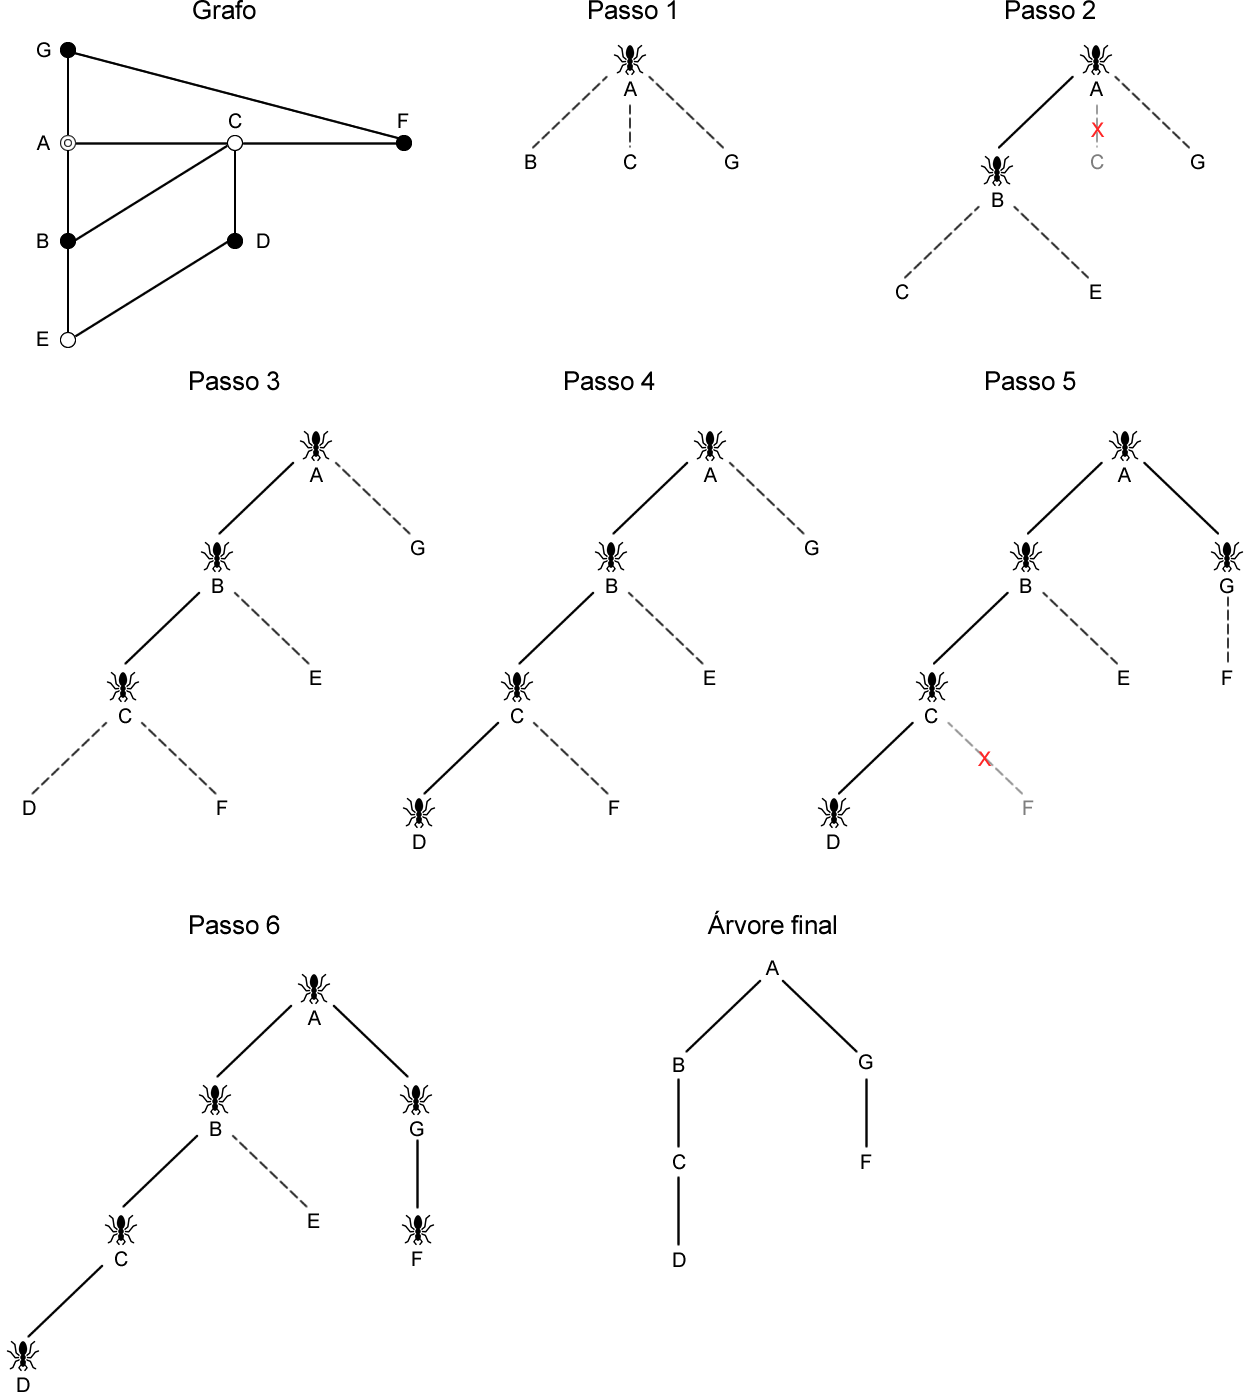
\includegraphics[width=1\textwidth]{cap_algoritmo-proposto/figs/exemplo-solucao}
	\caption{\label{fig_exemplo_solucao}Exemplo de como construir uma solução para o PRM}
\end{figure*}

Trabalhar com todas as arestas possíveis é demasiadamente caro e inviável para um algoritmo em que se deseja bom desempenho quanto ao tempo de execução. Por isso, trabalha-se com uma amostra da lista de exploração (linha 5 do algoritmo). Outro processo de simplificação também é empregado para evitar o crescimento exagerado de $Exp_a$ durante a etapa de exploração, nas linhas 12 a 16. Nesse processo, caso um novo vértice descoberto já seja atingível a partir de alguma aresta em $Exp_a$, mantém-se em $Exp_a$ apenas uma das arestas. Para escolher qual das arestas manter, calculam-se as probabilidades de acordo com os feromônios ($\tau$) e a heurística ($h$).

Com relação às heurísticas no PRM, uma função é construída para cada métrica de rede presente na formulação de objetivos. Por exemplo, no problema $P_4$, cujos objetivos envolvem as métricas custo, \textit{delay}, tráfego e capacidade, quatro heurísticas são criadas:

\[ \begin{cases} 
h_1(e) = 1 - custo(e) \\
h_2(e) = 1 - delay(e) \\
h_3(e) = 1 - trafego(e) \\
h_4(e) = capacidade(e)
\end{cases}
\]

Onde $custo(e)$, $delay(e)$, $trafego(e)$ e $capacidade(e)$ correspondem, respectivamente, ao valor normalizado entre 0 e 1 para o custo, \textit{delay}, tráfego e capacidade da aresta $e$. Na heurística $h_4$ não é feito o complemento da função, pois essa é a única métrica que deve ser maximizada.

\section{\textit{Framework} MACO/NDS}
\label{section_algoritmo_framework}

O MACO/NDS se baseia na ideia do AEMMD de se criar conjuntos de soluções não dominadas para diferentes combinações possíveis de objetivos, adaptando-a para um modelo de colônia de formigas.

A multiplicidade de objetivos impõe que algumas mudanças sejam feitas na ideia original do ACO. Isso envolve responder as seguintes perguntas:

\begin{itemize}
	\item Como representar os diferentes objetivos no depósito de feromônio?
	\item Como compor as múltiplas heurísticas em uma única função?
\end{itemize}

De acordo com \cite{Alaya2007}, essas questões podem ser resolvidas através de uma das seguintes opções:

\begin{itemize}
	\item \textbf{Várias colônias e múltiplos feromônios $(m+1, m)$:} considerando $m$ o número de objetivos, esse modelo utiliza $m + 1$ colônias de formigas e $m$ estruturas de feromônios. Cada colônia é associada a um único objetivo e otimiza apenas esse objetivo através de sua própria estrutura de feromônios. Uma colônia adicional, que representa o conjunto de todos os objetivos, utiliza os feromônios das outras colônias de forma aleatória. Ao criar uma solução, sorteia-se alguma das estruturas de feromônios para se utilizar a cada passo. Outra proposta, no modelo $(m+1, m)$ é utilizar a soma de todas as estruturas de feromônios ao criar uma solução na colônia extra. Quanto às heurísticas, cada colônia utiliza a função referente a seu objetivo, enquanto a colônia extra utiliza o somatório de todas as funções de heurística.
	\item \textbf{Colônia e feromônio únicos $(1,1)$:} este modelo utiliza apenas uma colônia de formigas e uma estrutura de feromônios. Assim como no modelo anterior, as heurísticas são somadas para montar uma solução. A estrutura única de feromônios representa todos os objetivos. A atualização dos feromônios se dá através de um arquivo que mantém todas as soluções não-dominadas encontradas. Toda solução não-dominada contribui com a mesma quantidade de feromônios, já que, de fato, são indiferenciáveis em termos de qualidade.
	\item \textbf{Única colônia e vários feromônios $(1,m)$:} considerando $m$ o número de objetivos, esse modelo utiliza uma colônia de formigas e $m$ estruturas de feromônios. Assim como nos demais modelos, as heurísticas são somadas para montar uma solução. A cada passo da construção da solução, sorteia-se aleatoriamente a estrutura de feromônios a se utilizar. Cada estrutura de feromônios representa um objetivo e sua atualização é feita a cada iteração do algoritmo, de acordo com a melhor solução encontrada considerando aquele objetivo.
\end{itemize}

Em \cite{Alaya2007}, os experimentos mostraram que o terceiro modelo ($1,m$) gera os melhores resultados quando aplicado ao problema da mochila multiobjetivo. Dentre os ACOs multiobjetivos investigados, o MOACS se encaixa na segunda abordagem (1,1), adaptando apenas o modo de lidar com a heurística (soma ponderada com pesos aleatórios), enquanto o MOEA/D-ACO adota a primeira estratégia, pois trabalha com múltiplas formigas e várias estruturas de feromônios, apesar da quantidade exata de formigas e tabelas de feromônios não ser ditada somente pelo número de objetivos (depende também do parâmetro $H$, ou número de divisões, passado ao algoritmo).

O algoritmo proposto nesta dissertação (MACO/NDS), não pertence a nenhuma das categorias apresentadas por \cite{Alaya2007}, mas se aproxima da estratégia (1,m), pois lida com uma única colônia e múltiplos feromônios. A grande diferença é que o número de estruturas de feromônio não é igual à quantidade de objetivos, mas ao número de possíveis combinações entre os objetivos, de forma semelhante ao que ocorre no AEMMD \cite{Lafeta2017}. Na verdade o modelo é (1, $|P|$), onde $P$ é o conjunto de subproblemas e seu tamanho é definido por:

\begin{equation}|P| = \sum_{i = 2}^m C_m^i\end{equation}

Sendo, $m$ a quantidade de objetivos considerados, $i$ a quantidade de objetivos considerados na combinação e $C$ a quantidade de possibilidades combinando os objetivos $i$ a $i$.

Além disso, o processo de cálculo da heurística e de atualização dos feromônios também se difere substancialmente da ideia original do modelo $(1,m)$. O MACO/NDS, se baseia na ideia de decomposição, ou seja, ao invés de trabalhar diretamente com todos os objetivos, o problema é atacado em várias frentes com quantidades reduzidas de funções. Desta forma, evita-se o problema de classificação da população devido ao alto número de soluções não-dominadas em espaços de dimensionalidade alta \cite{Deb2014}. Os feromônios no MACO/NDS são encapsulados por uma estrutura chamada ``subproblema'', que contém as seguintes propriedades: 

\begin{itemize}
	\item \textbf{Objetivos:} determina os objetivos do subproblema em questão. É um vetor binário de tamanho $m$ (número de objetivos), onde o bit 1 representa um objetivo que faz parte do problema e o bit 0 indica aqueles que não pertencem ao problema.
	\item \textbf{Feromônios:} corresponde aos valores dos feromônios em si, os quais são inicializados com o menor valor possível (parâmetro de entrada).
	\item \textbf{Arquivo:} conjunto de soluções não-dominadas que apareceram até o momento para o subproblema em questão.
	\item \textbf{Convergência:} indica a convergência do arquivo. Começa em 0 e incrementa em 1 sempre que o arquivo sofre alterações durante uma iteração (época).
	\item \textbf{$\beta$:} importância da heurística no cálculo de probabilidades ao construir uma solução. Um valor para $\beta$ é informado como parâmetro de entrada do MACO/NDS e representa o valor inicial desse parâmetro ($\beta$) em cada subproblema.
\end{itemize}

Cada subproblema é responsável por uma combinação de objetivos. O funcionamento básico do MACO/NDS é ilustrado na \autoref{img_fluxo_maconds} e descrito no \ref{alg_macod_geral}.

\begin{figure*}[!htbp]	
	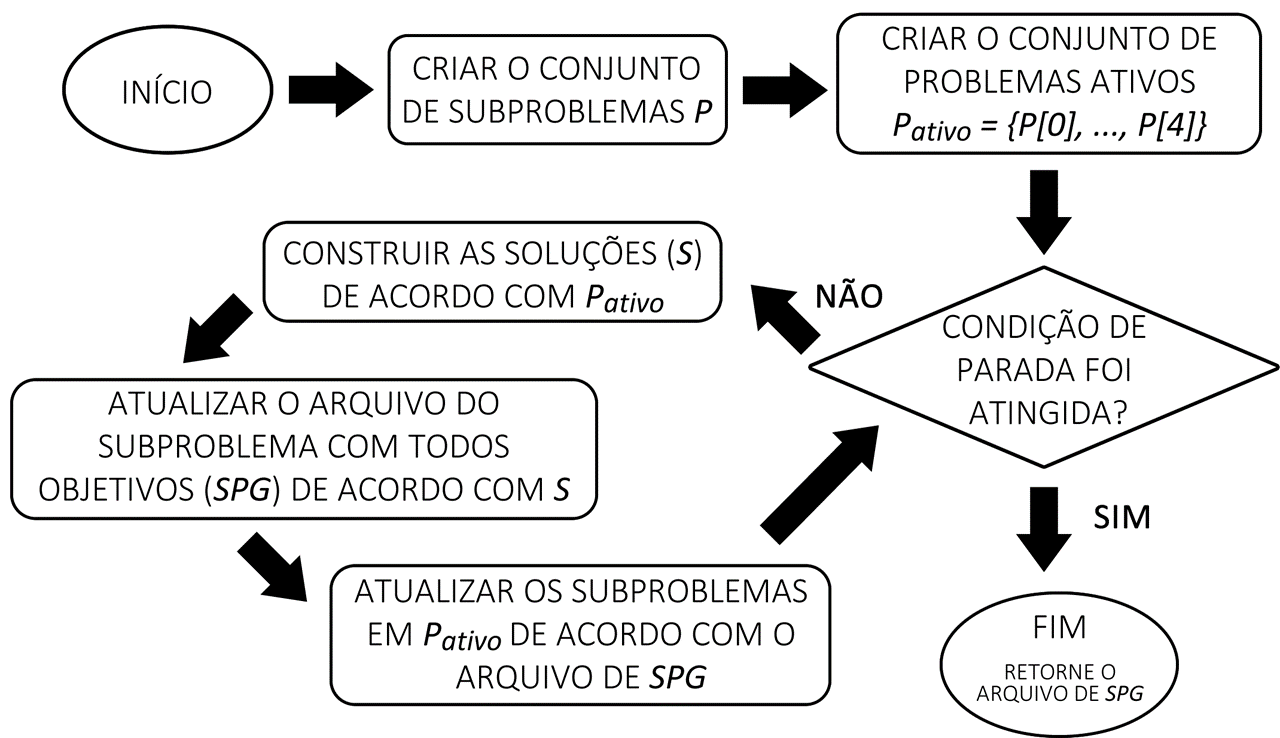
\includegraphics[width=1\textwidth]{cap_algoritmo-proposto/figs/fluxo-algoritmo-geral}
	\caption{\label{img_fluxo_maconds}Fluxo geral de execução do MACO/NDS}
\end{figure*}

\begin{algorithm}[!htbp]
	\caption{Algoritmo geral do MACO/NDS}
	\label{alg_macod_geral}
	\begin{algorithmic}[1]
		\State $P \gets criarSubproblemas()$
		\State $P_{ativo} \gets \{P[0], P[1], ..., P[4]\}$
		\State $sgi \gets tamanho(P) - 1$ // índice do subproblema geral
		\While{condição de parada não for atingida}
		\State $S \gets criarSolucoes(P_{ativo})$
		\State $atualizarArquivo(P[sgi], S)$
		\State $S_{nd} \gets P[sgi].arquivo$
		\State $atualizarSubproblemas(P_{ativo}, S_{nd})$
		\EndWhile
		\State \Return $S_{nd}$
	\end{algorithmic}
\end{algorithm}

O primeiro passo do MACO/NDS (linha 1 do Algoritmo \ref{alg_macod_geral}) é criar as estruturas de dados para os subproblemas $P = \{p_1, p_2, ..., p_i, ..., p_n\}$, uma para cada combinação possível de objetivos (análogo ao processo do AEMMD apresentado na seção \ref{section_aemmd}). Para um problema de seis objetivos ($m = 6$), por exemplo, são criados 57 subproblemas que decompõem o problema principal. São 57 subproblemas, pois, se $m = 6$, $|P| = \sum_{i = 2}^m C_m^i = 15 + 20 + 15 + 6 + 1 = 57$.

Os subproblemas são utilizados no processo de construção da solução e devem ser atualizados em toda iteração do algoritmo. Manipular todos os elementos de $P$ (57 subproblemas, no caso de seis objetivos) é computacionalmente caro e inviável. Por essa razão, define-se um número máximo de subproblemas para se trabalhar em um dado momento. Em ambos os problemas utilizados neste trabalho (PMM e PRM), foi utilizado um limite de cinco subproblemas ativos simultaneamente. A ordem de ativação dos elementos de $P$ é determinada pela sua ordem. Por isso, é importante a sequência em que as estruturas são criadas: os primeiros subproblemas instanciados são aqueles que representam um menor número de  objetivos, ou seja, combinações 2 a 2. Em seguida, instanciam-se os subproblemas de 3 objetivos e, assim por diante, até que o último subproblema, com o número total de objetivos, seja criado.

Na linha 2 do algoritmo, os cinco subproblemas mais simples são ativados (ou seja, as 5 primeiras combinações de objetivos). No processo de atualização (linha 8), assim que algum dos subproblemas passa a não contribuir para o conjunto de soluções, esse é desativado em favor do próximo subproblema. Dessa forma, o conjunto de soluções do MACO/NDS cresce gradualmente, partindo das decomposições mais simples, que utilizam um número menor de objetivos, em direção às mais complexas, que utilizam um número maior, até que seja ativado o subproblema que lida com todos os $m$ objetivos.

Na linha 3, a variável $sgi$ é usada para armazenar o índice do subproblema que considera todos os objetivos (último subproblema de P). O laço principal do ACO, descrito entre as linhas 4 e 9 do algoritmo, consiste em gerar soluções e atualizar as estruturas de subproblema. Inicialmente (linha 5), é construído o conjunto de soluções $S$ de acordo com os feromônios dos subproblemas em $P_{ativo}$, esse processo é detalhado na seção \ref{section_macod_solutions}. Na linha 6, o arquivo do último subproblema (com todos os objetivos) é atualizado com as soluções em $S$. Na linha 7, esse arquivo é armazenado em $S_{nd}$, como referência ao arquivo principal com todas as soluções não dominadas envolvendo o problema original (todos os objetivos). Por último, na linha 8, as soluções de $S_{nd}$ são utilizadas para atualizar cada uma das estruturas de subproblema em $P_{ativo}$. No final, o algoritmo MACO/NDS retorna todas as soluções não dominadas encontradas ($S_{nd}$).

\subsection{Construção das soluções}
\label{section_macod_solutions}

As soluções em colônias de formigas são construídas a partir dos feromônios do subproblema ativo ($P_{ativo}$), das heurísticas ($H$) e dos valores de $\alpha$ e $\beta$. Os feromônios são criados e atualizados no decorrer do algoritmo, enquanto os demais são parâmetros de entrada. A heurística é uma função que estima a qualidade de uma parcela da solução, ex: arestas em problemas que envolvam grafos, como o PRM, e itens em problemas representados por vetores, como o PMM. Enquanto o parâmetro $\alpha$ determina a importância do feromônio ao tomar uma decisão a respeito da composição da solução, $\beta$ representa a importância da heurística.

No MACO/NDS existem múltiplos feromônios (encapsulados pelas estruturas de subproblema) e heurísticas. Portanto, para que se possa construir uma solução, é necessário antes escolher quais valores de feromônio e qual função de heurística serão utilizados. 

Os subproblemas utilizados no processo de construção das soluções pelas formigas é a lista de subproblemas ativos do MACO/NDS ($P_{ativo}$). Ou seja, 5 subproblemas são utilizados por vez para construir o conjunto de soluções $S$ com $n$ elementos. Logo, cada subproblema servirá de base para construir $n/5$ soluções de $S$.

Com relação às heurísticas, o MACO/NDS utiliza o mesmo processo proposto em \cite{Riveros2016}. Admite-se um grau de importância para cada função: 0 (não importante), 1 (importante) ou 2 (muito importante). O valor de importância é sorteado para cada heurística e funciona como um peso. A função única utilizada para construir a solução é a soma ponderada das heurísticas considerando os pesos sorteados.

O processo geral para a construção das soluções pelas formigas é exposto no Algoritmo \ref{alg_macod_solucao}.

\begin{algorithm}
	\caption{Construção das soluções}
	\label{alg_macod_solucao}
	\begin{algorithmic}[1]
		\State $S \gets \emptyset$
		\For{$i \gets 0$ até $n$}
		\State $W \gets \emptyset$
		\For {$j \gets 0$ até $|H|-1$}
		\State $W[j] \gets random(0,2)$
		\EndFor
		\State $h(x) \gets \sum_{i \gets 0}^{|H|-1}\frac{H[i](x) * W[i]}{\sum\limits_{w \in W}w}$
		\State $p \gets P_{ativo}[i \pmod{|P_{ativo}|}]$
		\State $s \gets gerarSolucao(p.feromonios, h, \alpha, p.\beta)$
		\State $S \gets S \cup \{s\}$
		\EndFor
		\State \Return $S$
	\end{algorithmic}
\end{algorithm}

O Algoritmo \ref{alg_macod_solucao} apresenta o processo geral para se construir um conjunto de soluções. Na linha 1, $S$ é inicializado como um conjunto vazio. A partir da linha 2, um laço é executado para gerar todas as soluções necessárias. Nas linhas 3 a 6, $|H|$ valores entre 0 e 2 (inclusive) são sorteados para um vetor de pesos $W$. Na linha 7, é criada a função heurística correspondente à combinação de todas as heurísticas de acordo com os pesos sorteados. Na linha 8, $p$ recebe o subproblema que será utilizado na construção da solução $i$. A escolha do subproblema é feita de forma sequencial e circular, de modo a garantir uma distribuição uniforme entre os indivíduos do conjunto de soluções $S$. A nova solução é criada por uma formiga na linha 9 de acordo com os feromônios de $p$, a função heurística $h$, o parâmetro do $\alpha$ do algoritmo e o valor $\beta$ de $p$. Na linha 10, a nova solução é incluída no conjunto de soluções $S$. Por fim, na linha 12, retorna-se o conjunto $S$ de soluções.

Na linha 9 do algoritmo \ref{alg_macod_solucao} constrói-se a solução em si. Esse processo depende exclusivamente do problema em questão e representa a principal parte na elaboração do modelo para um algoritmo baseado em colônia de formigas. No caso do problema da mochila multiobjetivo, a estratégia utilizada é aquela descrita em \ref{section_algoritmo_pmm}. Para o problema do roteamento multicast, a estratégia de construção da solução foi apresentada em \ref{section_algoritmo_prm}.

\subsection{Atualização das estruturas de subproblemas}

O processo de atualizar as estruturas de subproblema a partir das novas soluções não dominadas encontradas (linha 8 do Algoritmo \ref{alg_macod_geral}) é mostrado com mais detalhes no Algoritmo \ref{alg_macod_dist}, que recebe como entrada o conjunto $P_{ativo}$ e o conjunto de soluções $S_{nd}$

\begin{algorithm}[!htbp]
	\caption{Atualização dos subproblemas}
	\label{alg_macod_dist}
	\begin{algorithmic}[1]
		\For{$i \gets 0$ até $|P_{ativo}|$}
		\State $a \gets P_{ativo}[i]$
		\State $dif = atualizarArquivo(a, S_{nd})$
		\State $A \gets dif.added$
		\State $R \gets dif.removed$
		\If{|A| > 0}
		\State $a.\beta \gets \beta$
		\State $depositarFeromonios(a, A)$
		\State $evaporarFeromonios(a, R)$
		\Else
		\State $a.convergencia \gets a.convergencia + 1$
		\State $a.\beta \gets a.\beta \times \beta_{inc}$
		\If{$a.convergencia > MAX_{convergencia}$}
		\State $P_{ativo}[i].convergencia \gets 0$
		\State $P_{ativo}[i] \gets proxima\_estrura\_feromonios$,
		\EndIf
		\EndIf
		\EndFor
	\end{algorithmic}
\end{algorithm}

O Algoritmo \ref{alg_macod_dist} mostra a atualização das estruturas de subproblema no MACO/NDS. O processo iterativo (linha 1) passa por todas as estruturas em $P_{ativo}$. Nas linhas 2 a 5, a estrutura atual é chamada de $a$ e seu arquivo é atualizado de acordo com as soluções no conjunto $S_{nd}$. Além disso, todas as soluções adicionadas ao arquivo são guardadas na lista $A$, enquanto todas as removidas são colocadas em $R$. As linhas 7, 8 e 9 são executadas apenas se o arquivo de $a$ foi atualizado. Na linha 7, o valor $beta$ de $a$ é reinicializado para o valor original (parâmetro $\beta$ do algoritmo); na linha 8, os valores de feromônio de $a$ são incrementados de acordo com as novas soluções ($A$); e na linha 9, os valores de feromônios de $a$ são decrementados de acordo com as soluções removidas ($R$). As operações das linhas 8 e 9 são detalhadas na seção \ref{section_macod_pheromones}, sobre a atualização dos feromônios. Os valores de feromônios são alterados apenas se o arquivo relacionado ao subproblema corrente ($a = P_{ativo}[i]$) tiver sido modificado. Por outro lado, caso o arquivo não tenha sofrido atualização, as linhas 11 a 16 são executadas. Na linha 11, a convergência de $a$ é incrementada em 1. Na linha 12, o valor $\beta$ de $a$ é modificado de acordo com a constante pré-definida $\beta_{inc}$. Como temos $\beta_{inc} > 1$, o valor de $\beta$ atual correspondente ao subproblema corrente é aumentado. A ideia é que se diminua a importância das heurísticas sempre que a busca parecer estagnada. Como na implementação utilizada neste trabalho os valores das heurísticas são normalizadas entre 0 e 1, para diminuir a importância da heurística, deve-se aumentar o valor de $\beta$, por isso $\beta_{inc} > 1$. O valor de $\beta_{inc}$ é um parâmetro que depende do problema. Nos nossos experimentos (descritos no capítulo \ref{chapter_experimentos}), o valor de $\beta$ aumenta em 10\% tanto no PMM quanto no PRM, ou seja, $\beta_{inc} = 1,1$. Caso novas soluções sejam encontradas, o valor $\beta$ associado ao subproblema corrente ($a.\beta$) volta ao valor inicial de $\beta$ (linha 7). Por último, nas linhas 14 e 15, se a convergência de $a$ atingiu o limite máximo $MAX_{convergencia}$, substitui-se a estrutura $a$ em $P_{ativo}$ pelo próximo $p_i \in P$, e reinicia-se o valor da convergência de $a$, de modo que possa ser reutilizado, caso necessário, no decorrer do algoritmo (isso acontece quando todos os subproblemas foram utilizados, mas a condição de parada não foi atingida). O valor da constante $MAX_{convergencia}$ utilizado neste trabalho foi 10.

\subsection{Atualização dos feromônios}
\label{section_macod_pheromones}

No MACO/NDS, a atualização dos valores de feromônio em um subproblema pode ser de dois tipos:

\begin{enumerate}
	\item \textbf{Depósito:} a partir de uma nova solução construída, adiciona-se uma quantidade $\delta$ ao feromônio correspondente a cada parcela da solução. No caso de um problema em grafos, por exemplo, para cada aresta da solução, incrementa-se em $\delta$ o feromônio daquela aresta. O depósito de feromônio ocorre quando novas soluções não-dominadas são encontradas.
	\item \textbf{Evaporação:} similar ao depósito, mas ao invés de incrementar o feromônio em $\delta$, decrementa-se. Ocorre quando uma solução é removida do arquivo em decorrência de uma nova solução melhor.
\end{enumerate}

A evaporação no MACO/NDS, diferentemente da maioria dos algoritmos baseados em ACO, não ocorre para todas as arestas (parcelas da solução) em todas as iterações. Ao invés disso, o feromônio só é decrementado quando uma solução passa a ser dominada (linha 9 do Algoritmo \ref{alg_macod_dist}). Essa evaporação seletiva poderia causar convergência prematura se usada na maioria dos ACOs, pois grande parte dos feromônios atingiriam valores muito altos antes da condição de parada ser atingida. Isso não acontece no MACO/NDS devido à troca das matrizes de feromônios utilizadas para construir as soluções, quando suas respectivas convergências ultrapassam o limiar estabelecido (linha 13 do Algoritmo \ref{alg_macod_dist}). Dessa forma, as matrizes de feromônios correspondentes a cada subproblema não ficam ativas tempo suficiente para se tornaram um problema no que se refere à convergência do algoritmo.

Dada uma solução $s$ do problema do roteamento multicast (PRM), se $s$ deve ser reforçada (depósito), cada aresta $e$ da árvore $s$ incrementa o valor correspondente na matriz de feromônios em um fator $\delta$. Matematicamente, o valor de $\delta$ é definido por:

\begin{equation}\delta(e) = (1 - pesos(e)) \times \rho\end{equation}

Sendo, $pesos(e)$ a média dos pesos normalizados na aresta $e$ e $\rho$ a taxa de evaporação (parâmetro do MACO/NDS). Por outro lado, se $s$ se tornou uma solução dominada (saiu do arquivo) e, por isso, deve ser desencorajada (evaporação), os valores na matriz de feromônios correspondentes às arestas de $s$ devem ser decrementados em $\delta$.

Dada uma solução $s$ do problema da mochila multiobjetivo (PMM), se $s$ deve ser reforçada (depósito), cada item $i$ de $s$ incrementa o valor correspondente no vetor de feromônios em um fator $\delta$. O cálculo de $\delta$ no PMM é dado por:

\begin{equation}\delta(i) = lucros(i) \times (1 - peso(i) / peso\_{max}) \times \rho\end{equation}

Onde, $lucros(i)$ é a média dos valores normalizados de lucro do item $i$, e $peso\_{max}$ é o maior peso dentre todos os itens. Se $s$ deve ser desencorajada (evaporação), os valores no vetor de feromônios correspondentes aos itens de $s$ devem ser decrementados em $\delta$.